In this paper, we introduce a variation of the skip-gram model which jointly learns 
distributed word vector representations and their way of composing to form phrase embeddings.
In particular, we propose a learning procedure that incorporates a phrase-compositionality
function which can capture how we want to compose phrases vectors from their component
word vectors. Our experiments show improvement in word similarity and analogy tasks and a dependency 
parsing task using the proposed joint models.
\section{Introduction}
Distributed word vector representations learned from large corpora of unlabeled data have been shown to be effective in
a variety of NLP tasks, such as POS tagging~\cite{collobert2011scratch}, parsing~\cite{chen2014fast,DurrettKlein2015}, 
language modeling~\cite{bengio2003neural,mnih2007three} and machine translation~\cite{devlin-EtAl:2014:P14-1,liu-EtAl:2014:P14-1,sutskever2014sequence,kalchbrenner2013recurrent}.
These vector representations are computed using co-occurrence statistics of words and their neighboring context words.


One of the most widely used approaches to learn these vector representations is the skip-gram model described in \namecite{Mikolov:2013} and \namecite{mikolov2013distributed}. 
The skip-gram model optimizes the probability of predicting words in the context given the current center word.  
Figure~\ref{fig:skip-gram} shows a standard skip-gram structure. 
\namecite{ling-EtAl:2015:NAACL-HLT} present a variation of skip-gram which captures the relative position of context words
by using a different weight matrix to connect the hidden layer to the context word at each relative position. 


While word embeddings are usually used to compose distributed representations for larger units,
this compositionality is not used during the whole learning procedure. \namecite{socher-EtAl:2013:ACL2013} use a recursive neural network
to learn weight matrices that capture compositionality.
However, these matrices are updated using backpropagation over syntatic nodes of a parse tree and the
learning procedure is limited to the substantially 
smaller number of labeled parse trees from the Penn Treebank. The phrasal information from the large unlabeled corpus is not utilized.


\namecite{DBLP:journals/corr/LebretC15} propose a learning schedule which learns distributed vector representations for words and phrases jointly.
However, in the optimization phase, they only maximize the correlation between the phrase representation and the component word representation, which 
does not fully capture the syntatic information of context. Recently \namecite{yu2015learning} propose a feature-rich compositional transformation (FCT) model
which learns weighted combination of word vectors to compose phrase vectors. 
%The combinational weights
%are constructed using features within the phrase and additional parameters are learned during the backpropagation procedure. 
During the learning procedure, the current phrase embedding is used to predict the context word
vectors in the output embedding space and they mainly focus on bigram \textit{NP}s.


In this paper, we extend the skip-gram model to utilize the phrase structure in a large corpus to capture phrase compositionality and the positional information
of both words and phrases. We jointly model words in the context of words and
phrases in the context of phrases. Additionally, we enforce a compositionality constraint 
on both the input and output phrase embedding spaces which indicates how
we build the distributed vector representations for phrases from their component word vectors.
%While the boundary information of phrases is not available in a large corpus, it does not
%take much effort to do phrase extraction using existing toolkits like \textit{senna}~\cite{collobert2011scratch}, or \textit{word2phrase}~\cite{mikolov2013distributed}.
Our results show that using phrase level context information can provide gains in both word similarity and analogy tasks and also
syntactic tasks like dependency parsing.
\section{Skip-gram model}
\label{sec:skip}
\begin{figure}[!tbp]
    \scalebox{0.5}{
\begin{subfigure}[b]{0.4\textwidth}
        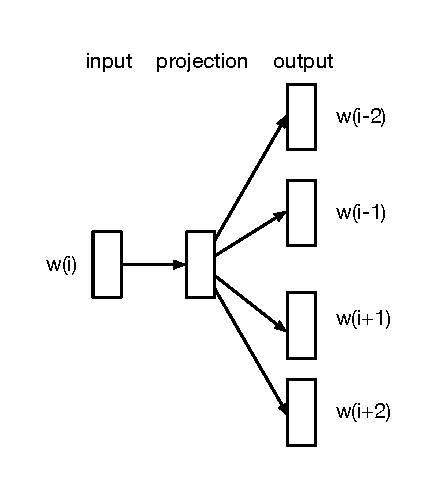
\includegraphics{./skip-gram.eps}
    \caption{word-level skip-gram}
    \label{fig:1a}
\end{subfigure}
\hfill
\begin{subfigure}[b]{0.55\textwidth}
    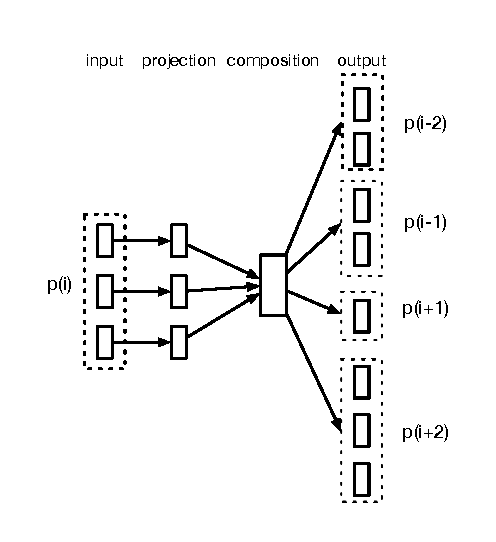
\includegraphics{./phrase-skipgram.eps}
    \caption{phrase-level skip-gram}
    \label{fig:1b}
\end{subfigure}
}
\caption{\small{Architecture of the skip-gram model.}}
\label{fig:skip-gram}
\vspace{-1em}
\end{figure}
The skip-gram model learns distributed vector representations for words by maximizing the probability of predicting
the context words given the current word. According to the \textit{word2vec} implementation of \namecite{mikolov2013distributed}, 
each input word $w$ is associated with a $d$-dimensional vector $v_w \in {\mathbb{R}}^{d}$ called the \textit{input embedding} and 
each context word $w_O$ is associated with a $d$-dimensional vector $v'_{w_O} \in {\mathbb{R}}^{d}$ called the \textit{output embedding}. $w, w_O$ are words from a vocabulary $V$
of size $W$. The probability of observing $w_O$ in the context of $w$ is modeled with a softmax function:
\begin{equation}
P(w_O | w) = \frac{\exp({v'_{w_O}}^T v_w)}{\sum_{i=1}^W \exp({v'_{w_i}}^T v_w)}
\end{equation}


The denominator of this function involves a summation over the whole vocabulary, which is impractical. One alternative 
to deal with the complexity issue is to sample several negative samples to avoid computing all the vocabulary. The objective
function after using negative sampling is:
\begin{equation}
\resizebox{.87\hsize}{!}{$\displaystyle
    E_w = \sum_{w \in s} (\log \sigma ({v'_{w_O}}^T v_w) + \sum_{i=1}^{K} \log \sigma (-{v'_{w_i}}^T v_w))
$}
\end{equation}
where $s$ is a chunked sentence. $w_i$, $i=1, 2, \ldots ,K$, are negative samples sampled from the following distribution:
\begin{equation}
P(w) = \frac{{\widetilde{P}(w)}^{\frac{3}{4}}}{Z}
\end{equation}
where $\widetilde{P}(w)$ is the unigram distribution of words and $Z$ is the normalization constant. The exponent $\frac{3}{4}$ is 
set empirically.
\section{Compositionality-aware skip-gram model}
\label{sec:compose}
%While word embeddings are usually used to compose distributed representations for larger units, 
%this compositionality has not been taken into account during the learning procedure of skip-gram model. 
To capture the way of composing phrase embeddings from distributed word vector representations, we extend the skip-gram model to include information from 
context of phrases and learn their compositionality from word vectors during the optimization procedure. Our phrase-level skip-gram structure is shown in
Figure~\ref{fig:1b}. %How we extract phrases in a large corpus is described in the next section.
\subsection{Phrase-level skip-gram model}
The word-level skip-gram model predicts the context words given the current word vector. Our approach further models the prediction of
context phrases given the vector representation of the current phrase vector (Figure~\ref{fig:1b}). Assume $v_p \in {\mathbb{R}}^d$ to be the $d$-dimensional 
input embedding for current phrase $p$ and $v'_{p_O}\in {\mathbb{R}}^d$ to be the output embedding for context phrase $p_O$. Using negative sampling, we model the phrase-level probability with:
\begin{equation}
\label{eq:phrase-skip}
\resizebox{.87\hsize}{!}{$\displaystyle
    E_p = \sum_{p\in s} (\log \sigma ({v'_{p_O}}^T v_p) + \sum_{i=1}^{N} \log \sigma (-{v'_{p_i}}^T v_p))
$}
\end{equation}
where $p_i$, $i= 1, 2, \ldots ,N$, are negative samples sampled according to the unigram probability of phrases raised to the same exponent $\frac{3}{4}$.


In this paper, we jointly model word-level skip-gram and phrase-level skip-gram for each sentence:
\begin{equation}
E = E_w + \beta E_p
\end{equation}
where $\beta > 0$ adjusts the relative importance of the word-level and the phrase-level skipgram.
\subsection{Compositionality model}
Assume a phrase $p$ is composed of words $w_1, \ldots ,w_{n_p}$, where 
$n_p$ is the number of component words. The vector representation for $p$ is computed as:
\begin{equation}
    v_p = \Phi(\oplus( \sigma(v_{w_1}), \ldots ,\sigma(v_{w_i})))
\end{equation}
where $v_p$ is the vector representation for $p$. The function $\sigma$ is a component-wise manipulation over each dimension.
%, which can be intepreted as adjusting the dimensional values to the phrase vector space.
The symbol $\oplus$ is an operator over the component word vectors, which can be \textit{linear combination, summation, concatenation} etc. 
The mapping function $\Phi$ is a linear or non-linear manipulation over the resulting vector after the $\oplus$ operation. The same composition function is used to compute 
the output phrase embeddings $v'_{p_O}$ and $v'_{p_i}$, except that the component word vectors are $v'_{w_i}$ instead of $v_{w_i}$.


To show the effect of modeling phrase embeddings, we experiment with a composition function where $\oplus$ is \textit{linear combination} and $\Phi$ is passing the resulting matrix to the left of a weight vector $l^p = [l_1^p , l_2^p, \ldots, l_{n_p}^p]$
associated with each phrase $p$ showing how we combine the component word vectors. 
\begin{equation}
\label{eq:linear}
\resizebox{.55\hsize}{!}{$\displaystyle
v_p = [\sigma(v_{w_1}), \ldots, \sigma(v_{w_{n_p}})] \begin{bmatrix} l_1^p \\ \vdots\\ l_{n_p}^p \end{bmatrix}
$}
\end{equation}
where the function $\sigma$ is a component-wise power function over vector $v=[v_1, \ldots, v_n]$:
\begin{equation}
    \sigma(v) = [\phi(v_1), \ldots, \phi(v_n)]
\end{equation}
where $\phi(v_i)=\textit{sign}(v_i)|v_i|^{\alpha}$, $\alpha\geq 1$, is a power function over each dimension. This manipulation can be interpreted as adjusting dimensional values of word vectors to the phrase vector space.


Stochastic gradient ascent is used to update the word vectors. In equation~\ref{eq:phrase-skip}, for each word $w_j$ in $p'$, either context phrase $p_O$ or negative 
phrase sample $p_i$, the gradient is:
\begin{equation}
%\frac{\partial E_p}{\partial v'_{w_j}} = l_j^{p'} (y-\sigma({v'_{p'}}^T v_p)) v_p \odot \triangledown \sigma(v'_{w_j})
    \frac{\partial E_p}{\partial v'_{w_j}} = \triangledown \sigma(v'_{w_j}) (l_j^{p'} (y-\sigma({v'_{p'}}^T v_p)) v_p) 
\end{equation}
where $y=1$ for each word in $p_O$ and 0 for each word in $p_i$. $\triangledown \sigma(v'_{w_j})$ is a diagonal matrix where the $i$-th diagonal value is $\phi'({v'_{w_j}}_i)$.
For each word $w_j$ in the current phrase $p$, the gradient is:
\begin{equation}
\resizebox{.85\hsize}{!}{$\displaystyle
\frac{\partial E_p}{\partial v_{w_j}} = \triangledown \sigma(v_{w_j}) (l_j^{p} ((1-\sigma({v'_{p_O}}^T v_p)) v'_{p_O} + \sum_{i=1}^{N} (-\sigma({v'_{p_i}}^T v_p)) v'_{p_i})) 
%\frac{\partial E_p}{\partial v_{w_j}} = (l_j^{p} ((1-\sigma({v'_{p_O}}^T v_p)) v'_{p_O} + \sum_{i=1}^{N} (-\sigma({v'_{p_i}}^T v_p)) v'_{p_i})) \odot \triangledown \sigma(v_{w_j})
$}
\end{equation}

\begin{table}
\centering
\begin{center}
\scalebox{0.75}{
\begin{tabular}{|l|l|l|l|l|l|l|} \hline
 length  & 1 & 2 & 3 & 4 & $\geq 5$\\ \hline
 frequency  & 525m & 137m & 62m & 22m & 15m\\ \hline
\end{tabular}}
\caption{\small{Statistics of phrase length distributions (m/million)}}
\label{tab:stats}
\end{center}
\end{table}
Similar compositionality functions trace back to \namecite{socher-EtAl:2013:ACL2013}, 
where $\oplus$ is \textit{concatenation} of component child node vectors (instead of word vectors) and $\Phi$ is a linear mapping from the
concatenated vector to a $d$-dimensional vector:
\begin{equation}
\resizebox{.45\hsize}{!}{$\displaystyle
v_p = [W_1^p,\ldots,W_{n_p}^p] \begin{bmatrix} \sigma(v_1) \\ \vdots \\ \sigma(v_{n_p}) \end{bmatrix}
$}
\end{equation}
where $\sigma$ is component-wise identity. $W_i^p \in {\mathbb{R}}^{m \times d}$ is a matrix associated with the vector representation of the $i$-th component word of
phrase $p$. 
%The weight matrices associated with context phrase $p'$ are ${W'}^{p'}_i, i=1,\ldots, n_{p'}$. 
Equation~\ref{eq:linear} can be seen as a special case of this composition when $m = d$, $W_i^p= l_i^p I_{d\times d}$ and the weight matrices are not updated during the procedure.

\subsection{Output phrase embedding space}
Following \namecite{ling-EtAl:2015:NAACL-HLT} in 
using different output embeddings at each relative position to capture order information of context words (we call this \textit{positional} model), 
we use separate output embeddings to capture phrase-compositionality (we call this \textit{compositional} model). That is, we have a separate component 
word vector $v''$ to compose the phrase vectors in the context 
and the negative samples instead of using $v'$.
The intuition of this choice is that we don't want the compositionality information in the context or negative sample layer 
to be distorted by word-level updates. 


We further extend the phrase-level skipgram to include the order information, which
uses different output word embeddings to compose phrases at each relative position. Phrases at the same relative position share the same
output embeddings (we call this model \textit{positional+compositional}).
Without loss of generality, we experiment with the composition
described in Equation~\ref{eq:linear}. The coefficients $l_i^p$s are set to be $\frac{1}{n_p}$.
%\subsection{Phrase extraction}
\section{Experiments}
\begin{table}
\centering
\begin{center}
\scalebox{0.55}{
    %\begin{tabular}{|l|p{3.1cm}>{\raggedleft\arraybackslash}|p{3.1cm}>{\raggedleft\arraybackslash}|p{3.1cm}>{\raggedleft\arraybackslash}|} \hline
    \begin{tabular}{|c|>{\raggedleft}p{3.5cm}|>{\raggedleft}p{2.9cm}|>{\raggedleft\arraybackslash}p{3.3cm}|} \hline
        Model  & \parbox{3.1cm}{denver\_nuggets} & \parbox{2.9cm}{fairy\_tale} & \parbox{3.3cm}{machine\_learning}\\ \hline
 word2vec  &\parbox{3.3cm}{dallas\_mavericks, colorado\_rockies, colorado\_avalanche, dallas\_desperados, colorado\_rapids} & 
 \parbox{3.1cm}{cautionary\_tales, folk\_tales, weird\_tales, strange\_tales, some\_tales}& 
 \parbox{3.3cm}{virtual\_machines, turing\_machines, time\_machines, sewing\_machines, intelligent\_machines}\\ \hline
 compositional  &\parbox{3.5cm}{seattle\_supersonics, dallas\_mavericks, philadelphia\_76ers, colorado\_rockies, \small{minnesota\_timberwolves}} &
 \parbox{3.1cm}{folk\_tales, ghost\_story, love\_story, arthurian\_legend, bedtime\_story} &
 \parbox{3.3cm}{computer\_skills, cognitive\_skills, computer\_vision, learned\_behavior, \small{mathematics\_and\_computer\_science}} \\ \hline
\end{tabular}}
\caption{\small{Examples of nearest neighbors using word2vec and using additional compositional model}}
\label{tab:neigh}
\end{center}
\end{table}
\label{sec:experiment}
We use the \textit{senna} toolkit~\cite{collobert2011scratch} to chunk our data,
which identifies the constituent chunks in each sentence. Even though the chunking model is 
not trained in the same domain, the chunking result does not degrade much 
for the simplicity of the task itself. We run the chunker on 20 CPUs, and it takes less
than 2 hours to chunk the Wikipedia 2010 corpus we use. %data size description here
The extracted phrases are labeled with \textit{NP, VP, PP}s etc. The statistics of the lengths of the extracted phrases 
is shown in Table~\ref{tab:stats}.


We train the skip-gram model with negative sampling using \textit{word2vec} as our baseline. We used an April 2010 snapshot of the Wikipedia corpus~\cite{wiki2010}, which contains approximately 2 million articles and 990 million tokens. 
We remove all words that have a frequency less than 20 and use a context window size of 5 (5 words before and after the word occurrence). 
We set the number of negative samples to be 10 and the dimensionality of vectors to be 300. 
For phrase-level skip-gram, we also use a context window size of 5 (5 phrases before and after the phrase occurrence).
%the phrase occurrence).

\begin{table}
\centering
\begin{center}
\scalebox{0.70}{
\begin{tabular}{|l|l|l|l|l|} \hline
            & word353 & men & SYN & MIXED \\ \hline
 word2vec  & 0.722 & 0.758 & 69.9      & 77.8  \\ \hline
positional & 0.692 & 0.744 & 71.2 & 79.7 \\ \hline
compositional &  \textbf{0.735}  & \textbf{0.763}   & 70.6   & 79.2 \\ \hline
compositional+positional & 0.704 & 0.746 & \textbf{72.0} & \textbf{80.5} \\ \hline
\end{tabular}}
\caption{\small{Comparison of word-level tasks, including word similarity, analogy.}}
\label{tab:word-task}
\end{center}
\end{table}
\subsection{Phrase nearest neighbors}
Table~\ref{tab:neigh} shows some phrases and their similar phrases (nearest neighbors). Following the ngram-to-ngram settings of~\namecite{yu2015learning}, 
we consider nearest neighbors that differ by more than one word. The word2vec phrase vectors are composed using summation. For word2vec, we can see that phrase vectors can be
greatly biased by one component word. As \textit{colorado} is similar to \textit{denver} (so does \textit{tales} to \textit{tale} and \textit{machines} to \textit{machine}), 
the nearest neighbors tend to be phrases that have this similar word, even though the phrase meaning is very different.
Using the compositional model, it is more likely to find phrases that have similar phrasal meanings. For example, the nearest neighbors of
\textit{denver nuggets} are mostly NBA teams. The model also find phrases of story types for \textit{fairy tale}
and related phrases like \textit{compute vision} and \textit{math and computer science} for \textit{machine learning}.


\subsection{Word similarity and word analogy}
We first consider word similarity and analogy tasks for evaluating the quality of word embeddings.
Word similarity measures Spearman's correlation coefficient between the human scores
and the embeddings' cosine similarities for word pairs. Word analogy measures the accuracy on
syntactic and semantic analogy questions. 


We evaluate similarity on two tasks, WordSim-353 and men, 
respectively containing 353 and 3000 word pairs. 
We use two word analogy datasets that we call SYN (8000 syntactic analogy questions) and MIXED (19544
syntactic and semantic analogy questions).


On the WordSim-353 task, \namecite{neelakantan-EtAl:2014:EMNLP2014} reported a Spearmans correlation of 0.709, while their word2vec baseline is 0.704.
From Table~\ref{tab:word-task}, we can see that positional information actually degrades the performance on the similarity task, while only adding compositional information
performs the best.
For syntactic and mixed analogy tasks which involves
syntax information, we can see that using phrase-level skip-gram and positional information both help and combining both gives the best performance. 
\subsection{Dependency parsing}
\begin{table}
\centering
\begin{center}
\scalebox{0.8}{
\begin{tabular}{|l|l|l|l|l|} \hline
    & \multicolumn{2}{l|}{Dev} & \multicolumn{2}{l|}{Test} \\ \hline
   & UAS & LAS & UAS      & LAS  \\ \hline
   word2vec  & 92.21 & 90.83 &  91.91     & 90.54  \\ \hline
  compositional & 92.34  & 90.91  &  92.02     &  90.64 \\ \hline
 positional & 92.29 & 90.88 & 92.05 & 90.67  \\ \hline
    compositional+ positional & \textbf{92.39} & \textbf{90.91} & \textbf{92.19} & \textbf{90.82} \\ \hline
\end{tabular}}
\caption{\small{dependency parsing results on PTB using different embeddings}}
\label{tab:dependency-task}
\end{center}
\end{table}
The evaluation on dependency parsing is performed on the English PTB, with the standard train, dev and
test splits with Stanford Dependencies. We use a neural network as described in \namecite{chen2014fast}. 
As we are using embeddings with a different dimensionality, we tune the hidden layer size and 
learning rate parameters for the neural network parser by grid search for each model and train for 15000 iterations. 
The other parameters are 
using the default settings. Evaluation is performed with the labeled (LAS) and unlabeled
(UAS) attachment scores. We run each parameter setting for 3 times and then average to prevent randomness.


Table~\ref{tab:dependency-task} shows the performance. 
We can see that combining phrase-level skip-gram and 
positional information consistently outperforms the baseline results.
\section{MCMC sampling}
\subsection{Joint model}
The extracted phrases using \textit{senna} suffer from the small average length for each phrase. We can see from 
Table~\ref{tab:stats} that most of the phrases are of length 1 and compositionality is used in very limited places.
Another problem with such kind of phrases is that the phrase boundaries are fixed and there is no way learning compositionality
between two adjacent phrases, especially cases where different chunkings are also valid phrases. For example,
\textit{new zealand} and \textit{new zealand islanders} are both valid phrases, while \textit{senna} would chunk \textit{new zealand}
as a phrase and \textit{islanders} as the second phrase. 


MCMC algorithms have been used to extract phrases by iteratively going through the unlabeled data and sample from left to right, one variable at a time
at each sentence. Usually a nonparametric bayesian model based on a nonparametric prior, such as Dirichlet Process, is used to smooth the distribution of
the data and avoid overfitting. The resulting posterior distribution is usually of the same family of distribution as the prior and thus 
has a closed-form solution. During the sampling procedure, the boundary variables would be sampled according to the posterior distribution and the phrases
in a sentence would vary whenever some of the boundary variables are flipped during the sampling procedure.


Therefore, we propose a joint MCMC sampling and compositionality learning model for phrase extraction and way of composing phrase embeddings. We use a log bi-linear
model to compute the probability of contexts given the phrase sequence:
$$P({\bf b},{\bf c}|{\bf w})= \frac{1}{Z}e^{\sum_i v'_{c_i} \cdot v_{p_i}}$$
where ${\bf w}$ is the word sequence and ${\bf b}$ is the binary sequence which models the boundary information for each phrase in the sequence and ${\bf c}$ is the context sequence for the phrases in the sequence.
At each position $j$, we sample its binary value:
$$b_j \propto e^{\sum_i v'_{c_i} \cdot v_{p_i}}$$
In practice we don't have to compute all the terms in the summation as most of them are not affected by the choice $b_j$. The terms that needs to be recomputed
involves the phrases that are affected by $b_j$: $(p_1, p_2)$ when $b_j=1$ and $p_3$ when $b_j=0$. 


After we have sampled the boundary variable $b_j$ and whenever we have reached a new phrase, we use the new phrase to predict its context. This can be done using
the compositional skip-gram model we have introduced before and the vectors are updated during the procedure. As for the update, we consider a few choices for the time
of vector update: 1. whenever a binary variable is flipped. 2. whenever we have reached the end of a phrase (sampled a binary value 1). 3. update when the boundary for the
whole sentence is decided.
\begin{algorithm}[t]
\small
\caption{A joint model for phrase extraction and compositionality learning}
\begin{algorithmic}[1]
\STATE{Initialize binary variables $b_1,\cdots, b_n$}
\FOR{$iter = 1,\cdots , T$:} 
    \FOR{$s = 1, \cdots, S$:}
        \FOR{$j = 1,\cdots , n$:}
            \STATE{Let $(p_1, p_2)$ be the two phrases when the $b_j=1$ and $p_3$ be the phrase when $b_j=0$}
            \STATE{Sample $b_j \propto e^{\sum_i v'_{c_i} \cdot v_{p_i}}$}
            \IF{$b_j = 1$}
                \STATE{Update $v_w$ for $w\in p_1$ according to the compositionality model}
            \ENDIF
        \ENDFOR
    \ENDFOR
\ENDFOR
\end{algorithmic}
\label{alg:joint}
\end{algorithm}
\subsection{Phrase independence variation}
In the previous section, we have modeled the probability of the whole sequence as a log bi-linear model. Here we consider factorizing the probability into product of probility of individual phrases.
$$P({\bf b},{\bf c}|{\bf w}) = \prod_i P(c_i| p_i) $$
where $P(c_i| p_i)$ is modeled with the standard skip-gram model.
$$P(c_i| p_i) = \prod_{p_j in c_i} \frac{1}{Z} e^{v'_{p_j} v_{p_i}}$$
where $Z$ is the normalization constant which sums over the whole phrase vocabulary $Q$.
$$Z = \sum_{p \in Q}e^{v'_p v_{p_i}}$$
The summation over the whole vocabulary is impractical. One alternative is to use negative sampling which approximate the sum over the whole vocabulary with a few samples.
$$Z = \sum_{j} ^{v'_{p_j} v_{p_i}}$$
where $p_j$s are negative samples sampled from the same uniform distribution described in the previous sections.


We sample the binary value $b_j$ according to the following probabilities:
$$P(b_j = 1) \propto P(c_1 | p_1) \cdot P(c_2 | p_2) \cdot P(c')$$
$$P(b_j = 0) \propto P(c_3 | p_3)\cdot P(c")$$
where $P(c')$ and $P(c")$ evaluate the change of contexts for the surrounding phrases when the binary value varies.

\section{Evaluation}
We evaluate results on the phrase similarity task described in~\namecite{Mitchell08vector-basedmodels}.

\section{Conclusion}
In this section, we have introduced a joint model for learning phrase embeddings and phrase compositionality. To overcome the limits of the the short length of each phrase and to increase flexibility of 
phrase boundaries, we propose an MCMC sampling schedule for additionally learning phrase boundary information.
